\documentclass{beamer}
\usepackage[utf8]{inputenc}
\usepackage[T1]{fontenc}
\usepackage[frenchb]{babel}

\usetheme{Madrid}
\usecolortheme{whale}
\beamertemplatenavigationsymbolsempty

\title{Recalage et fusion de modèles numérisés tridimensionnels de grande taille}
\subtitle{MEMO-F-403 - Préparation au mémoire}
\author{Tim Lenertz}
\date{\today}
\institute{ULB}

\maketitle

\begin{document}

\begin{frame}
\frametitle{Introduction}
	\begin{itemize}
	\item \textbf{Nuage de points}\\
		= points sur surface d'objet scanné
	\item Pris par scanner LIDAR, photogrammétrie
	\item Attribués par couleur RGB, température, intensité, etc.
	\item Documentation 3D \\
		(sites archéologiqes, bâtiments, terrain, dent, ...)
	\end{itemize}
\end{frame}

\begin{frame}
\frametitle{Nuage de points - Exemple 1}
	\center
	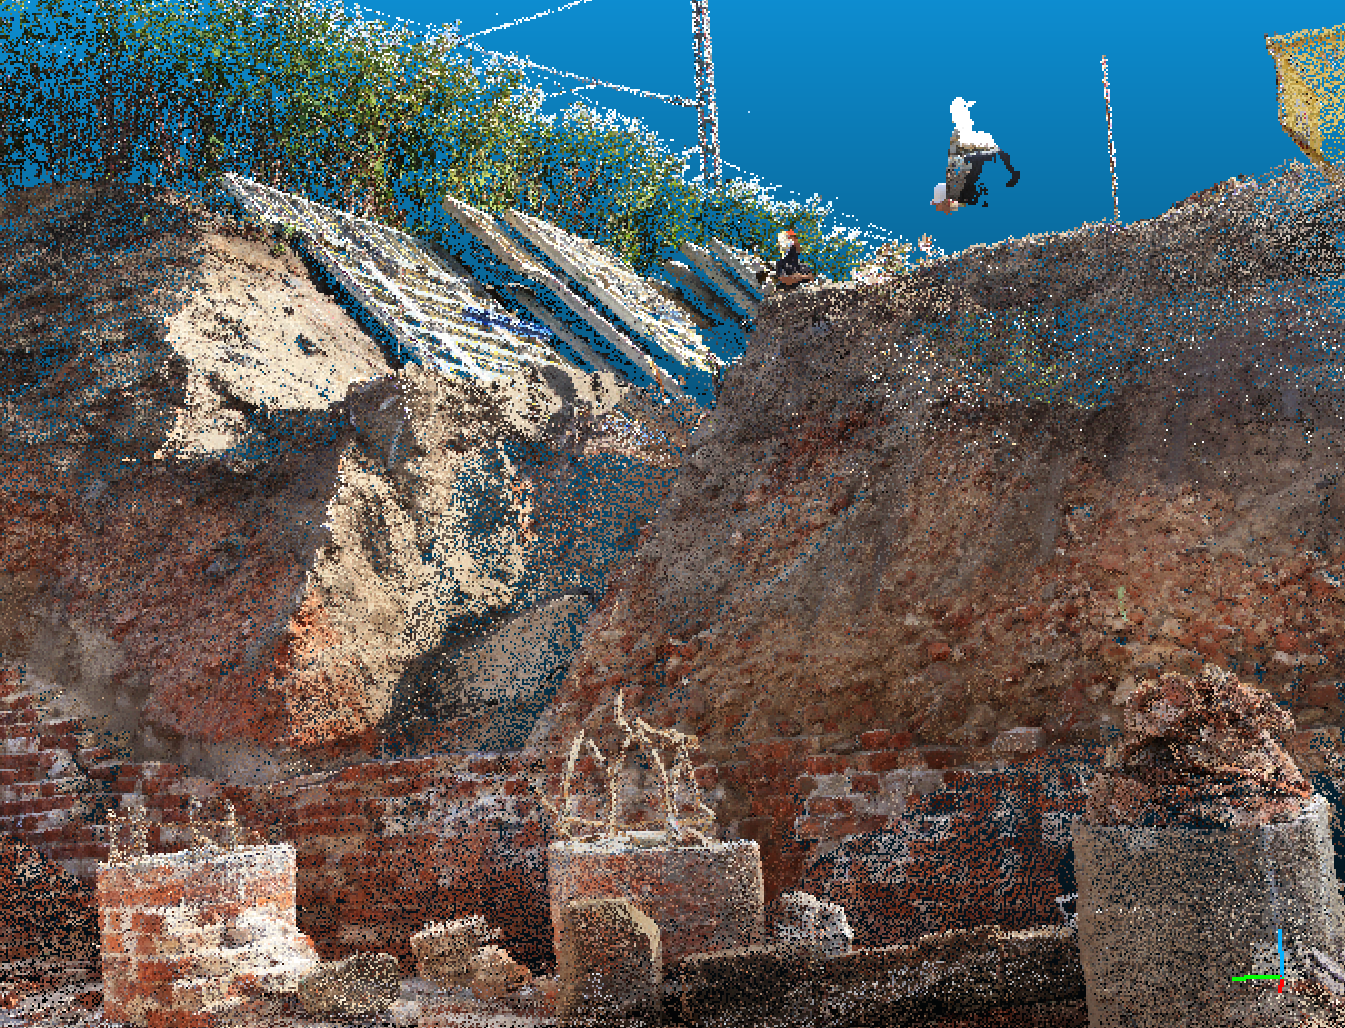
\includegraphics[width=.8\textwidth]{tower_screenshot.png} \\
	\footnotesize{Modèle de Jacobs University Bremen gGmbH}
\end{frame}

\begin{frame}
\frametitle{Nuage de points - Exemple 2}
	\center
	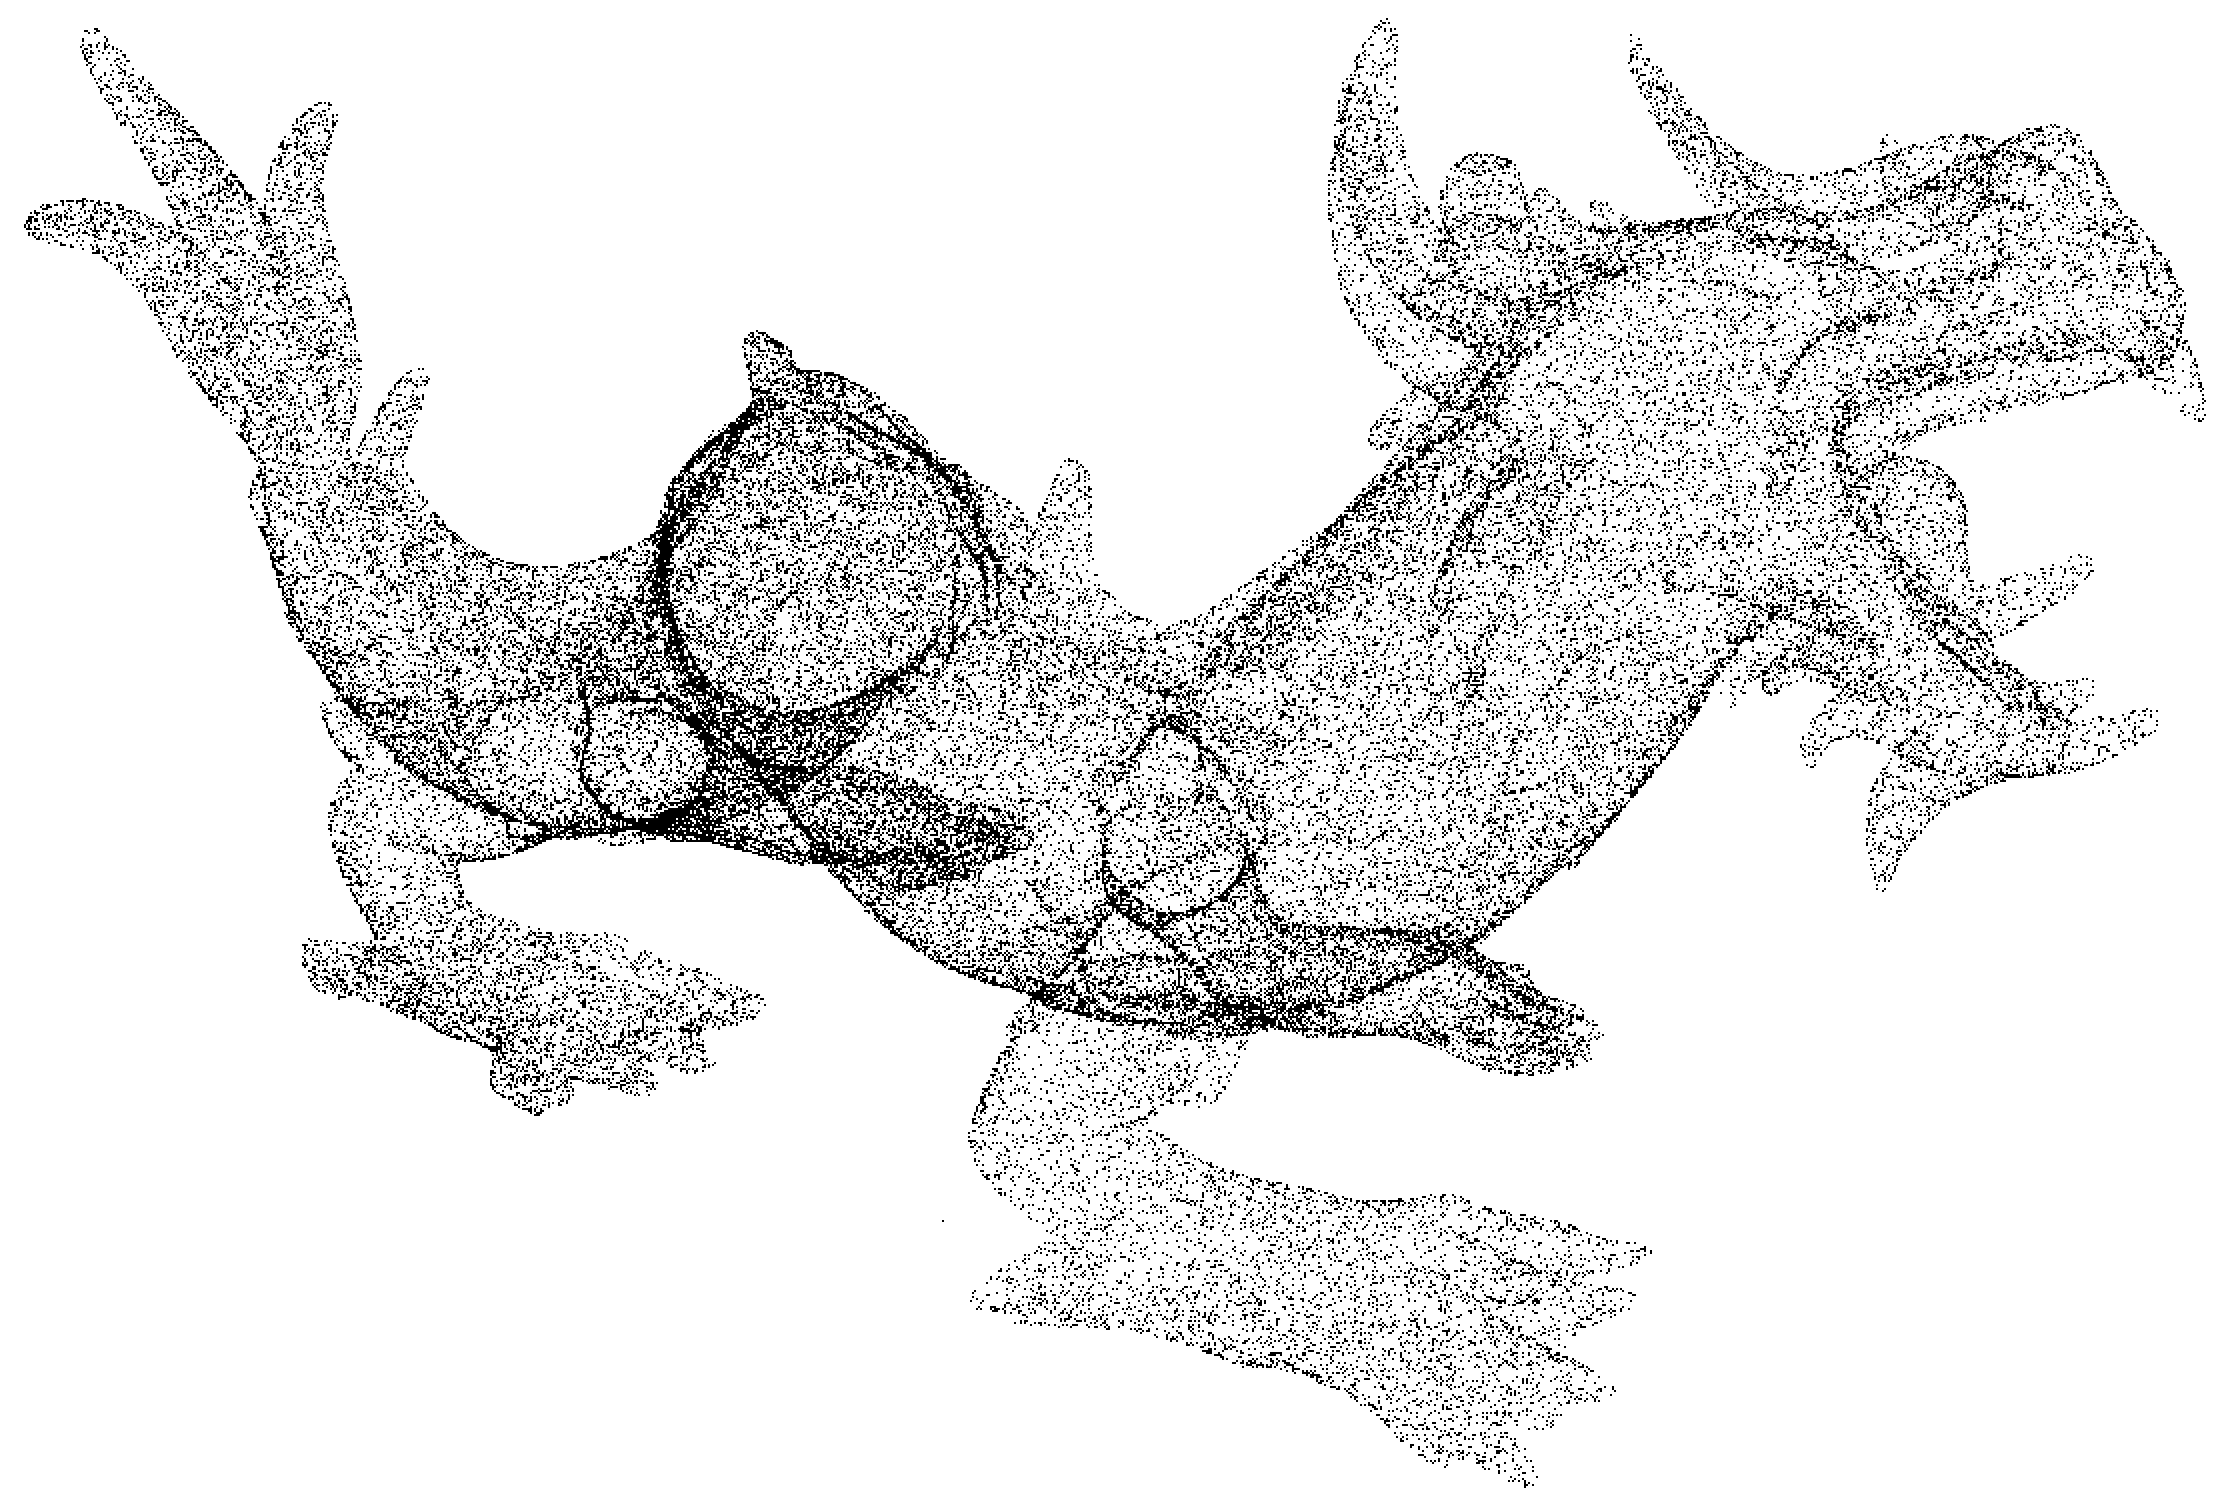
\includegraphics[width=.9\textwidth]{dragon_screenshot.png} \\
	\footnotesize{Modèle de Stanford Computer Graphics Laboratory}
\end{frame}

\begin{frame}
\frametitle{Scans bruts $\rightarrow$ modèle final}
	\begin{itemize}
	\item 
	\end{itemize}
\end{frame}

\begin{frame}
\frametitle{Recalage - Exemple}
	\center Recalage de 4 scans \footnotesize{\cite{Maka2006}}
	\vspace{1cm}
	\begin{columns}
	\begin{column}[T]{.5\textwidth}
		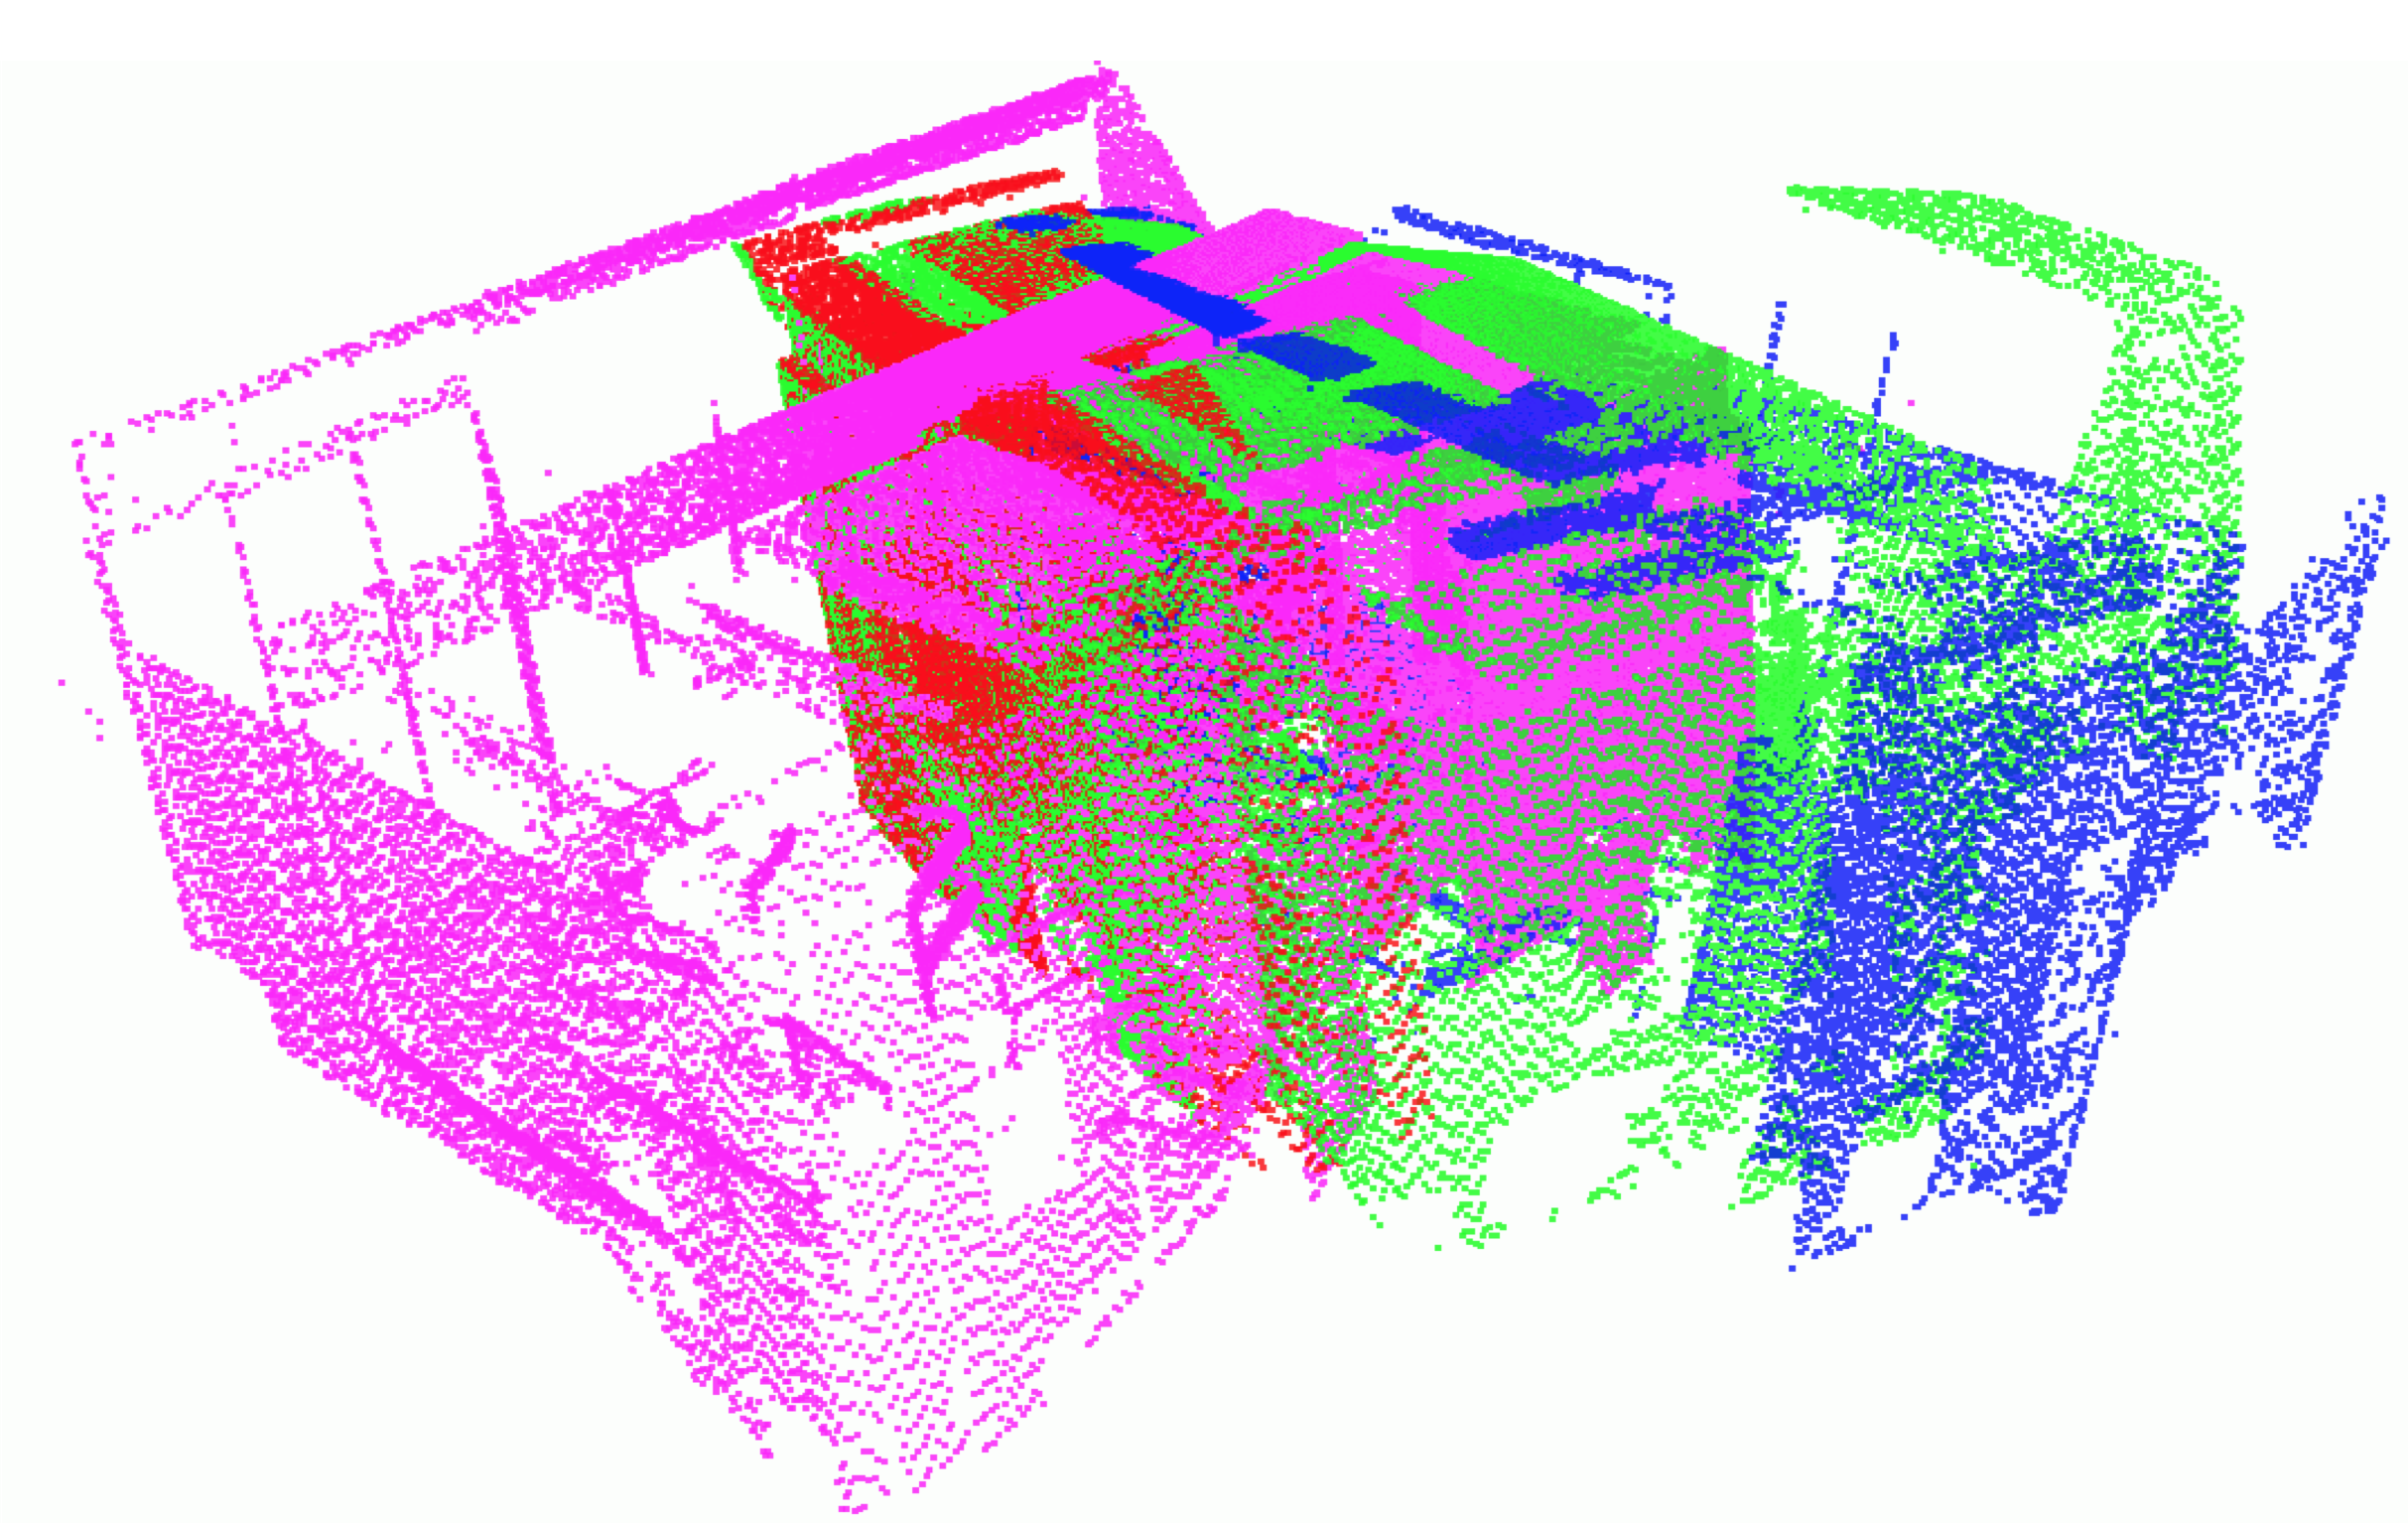
\includegraphics[width=\textwidth]{pre_reg.png}
		\center \Large{Avant}
	
	\end{column}
	\begin{column}[T]{.5\textwidth}
		\includegraphics[width=\textwidth]{post_reg.png}
		\center \Large{Après}
	\end{column}
	\end{columns}
\end{frame}

\bibliographystyle{plain}
\bibliography{../references}

\end{document}
